

%\documentclass[a4paper]{jarticle}


\section{mdtree.rb PMMLによる決定木モデルの描画\label{sect:mdtree}}
\index{mdtree@mdtree}
本コマンドは、PMML(Predictive Model Markup Language)で記述された決定木モデルをD3ライブラリによりHTML文書として視覚化する。
\verb|mbonsai|コマンド用の出力結果を視覚化する目的で作成したコマンドであるが、
他のソフトウェアで生成される決定木のPMMLデータであっても視覚化できるであろう。
PMMLでは数値とカテゴリの分岐ルールの記述方法は定義されているが、
\verb|mbonsai|で扱う系列パターンの有無の記述は定義されていない。
そのため、\verb|mbonsai|では、系列パーンによる分岐を記述するための拡張タグを定義しており、
本コマンドもその拡張タグに対応して決定木を視覚化できる。

\verb|mbonsai|で決定木を構築してから本コマンドで視覚化する一連の流れを以下に例示する。

\begin{table}[htbp]
\begin{center}
\begin{tabular}{c}

\begin{minipage}{0.5\hsize}
\begin{center}
\caption{入力データdat1.csv。全データは例を参照のこと。\label{tbl:mdtree_input1}}
{\small
\begin{tabular}{crlc}
\hline
性別&来店距離&購入パターン&入院歴 \\
\hline
男&1.2&ABCAAA&あり\\
男&10.5&BCDADD&あり\\
男&0.5&AAAA&なし\\
男&2.0&BBCC&なし\\
男&3.1&DEDDA&あり\\
女&0.7&CCCAA&なし\\
女&1.5&DDDEEE&あり\\
女&2.6&BACD&あり\\
女&3.5&ABBB&あり\\
女&4.0&DDDD&あり\\
女&2.1&DEDE&なし\\
:&:&:&:\\
\hline
\end{tabular} 
}
\end{center}
\end{minipage}

\end{tabular} 
\end{center}
\end{table} 

表\ref{tbl:mdtree_input1}に示されるデータを訓練データとして\verb|mbonsai|コマンドで決定木を構築する。
決定木は、\verb|O=|に指定したディレクトリにPMMLファイル\verb|model.pmml|として保存されている。
%ファイルの内容の詳細については\verb|mbonsai|のマニュアルを参照されたい。

\begin{Verbatim}[baselinestretch=0.7,frame=single]
$ mbonsai c=入院歴 n=来店距離 p=購入パターン d=性別 i=dat1.csv O=outdat
#END# kgbonsai O=outdat c=入院歴 d=性別 i=dat1.csv n=来店距離 p=購入パターン; IN=81;
$ ls outdat
alpha_list.csv model.pmml     model.txt      model_info.csv param.csv      predict.csv
\end{Verbatim}

そして、\verb|model.pmml|を視覚化するには以下のように本コマンドを実行すればよい。
出力された\verb|model.html|をブラウザで描画したものを図\ref{fig:mdtree_tree_1}に示す。

\begin{Verbatim}[baselinestretch=0.7,frame=single]
$ mdtree.rb i=outdat/model.pmml o=model.html
#END# mdtree.rb i=outdat/model.pmml o=model.html;
$ open model.html # macの場合はhtmlファイルをopenすればブラウザが起動され描画される
\end{Verbatim}

\begin{figure}[htbp]
\begin{center}
\begin{tabular}{c}

\begin{minipage}{0.9\hsize}
\begin{center}
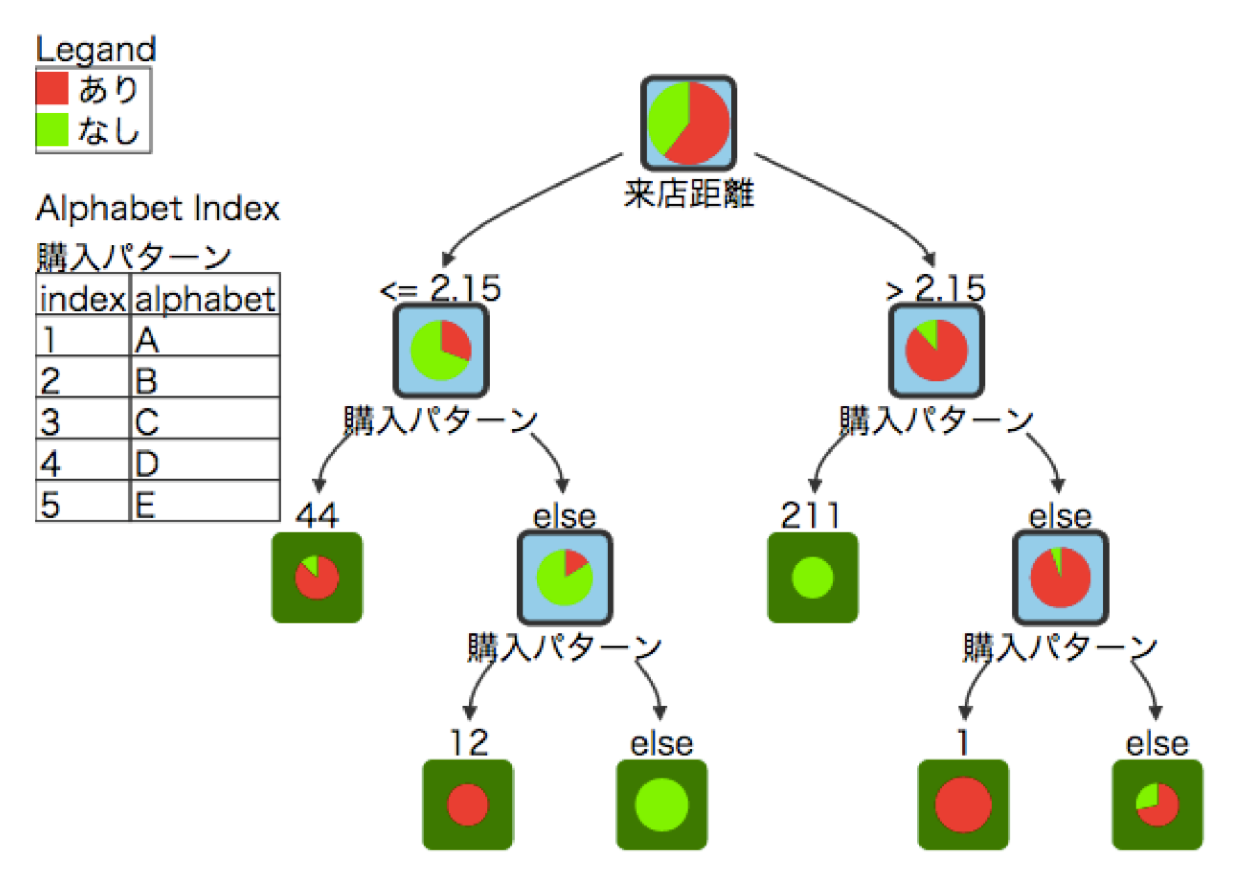
\includegraphics[scale=0.5]{figure/tree_1.eps}
\caption{本コマンドによる決定木の描画。
接点内の円グラフは、クラスの分布を示している(色は凡例に表示)。
背景が水色の節点は中間節点を、緑色の節点は葉節点を表している。
節点の直ぐ下には分岐に使う項目名が閉められており、節点の直ぐ上には分岐のルールが示されている。
例えば、最上位の節点では、来店距離が2.15以下であれば左に、2.15より長ければ右に分岐する。
系列パターンの場合は、そのパターンを含めば左に、含まなければ右に分岐する。
例えば、上から2段目の左の節点は、購入パターンに"44"を含んでいれば左に、含まなければ右に分岐することを意味している。
また、系列パターンの文字は、図の左上に示されたalphabet-indexの対応表におけるindexに示されている。
\label{fig:mdtree_tree_1}}
\end{center}
\end{minipage}

\end{tabular}
\end{center}
\end{figure}

また、\verb|mbonsai|で構築される決定木には最大木が保存されているので、
枝刈り度を\verb|alpha=|で指定することで枝刈りされた決定木を描画することもできる。
\verb|alpha=|は0以上の実数で、大きくすると枝が多く刈られる。
\verb|alpha|を指定しなかった場合、\verb|mbonsai|で交差検証を指定しなければ、
\verb|alpha=0.01|が指定されたことになり、交差検証を指定していれば、誤分類率最小のモデルが描画される。

図\ref{fig:mdtree_tree_2}に、\verb|alpha=0.1|で枝刈りした決定木を示す。
\begin{Verbatim}[baselinestretch=0.7,frame=single]
$ mdtree.rb alpha=0.1 i=outdat/model.pmml o=model2.html
#END# mdtree.rb alpha=0.1 i=outdat/model.pmml o=model.html;
$ open model2.html # macの場合はhtmlファイルをopenすればブラウザが起動され描画される
\end{Verbatim}

\begin{figure}[htbp]
\begin{center}
\begin{tabular}{c}

\begin{minipage}{0.5\hsize}
\begin{center}
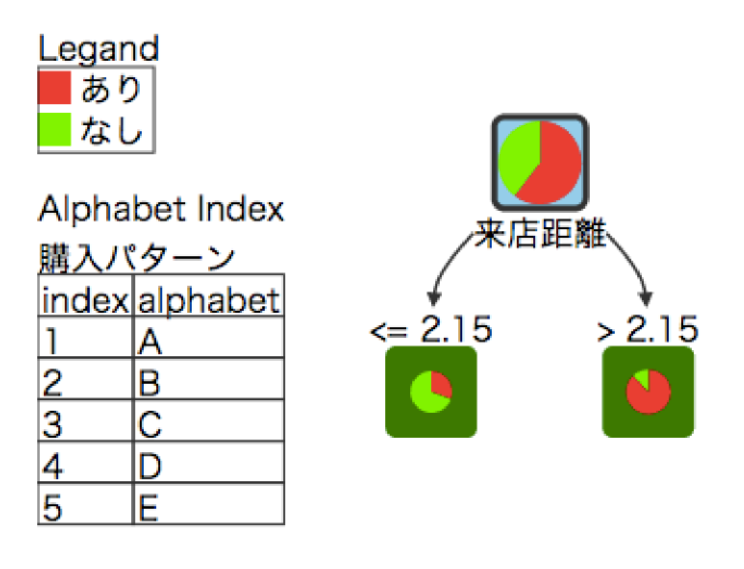
\includegraphics[scale=0.5]{figure/tree_2.eps}
\caption{枝刈り度alpha=0.1で描画した決定木\label{fig:mdtree_tree_2}}
\end{center}
\end{minipage}

\end{tabular}
\end{center}
\end{figure}

\subsection{Rとの連携}
統計解析パッケージRには多くの決定木構築パッケージが用意されている。
以下では、\verb|rpart|で構築した決定木を本コマンドで描画する方法を解説する。

%まずはRを起動し、rpartにより決定木をPMMLで保存するまでの一連の手順を以下に示す。
以下では、アヤメデータセット(\verb|iris|)と前立腺がんデータセット(\verb|stagec|)の2つのデータセットから
決定木を構築するRスクリプトである。
そこでは、決定木を構築する\verb|rpart|ライブラリとモデルをPMML出力する\verb|pmml|ライブラリを最初に読み込んでいる。
データセットの内容および決定木モデルの構築方法についての詳細は省略する。
最終的に、アヤメの決定木と前立腺がんの決定木が、
それぞれPMMLファイル\verb|model_r1.pmml|、\verb|model_r1.pmm2|として出力される。

\begin{Verbatim}[baselinestretch=0.7,frame=single]
library(pmml)
library(rpart)
iris.rp=rpart(Species~.,data=iris)
sink("model_r1.pmml")
pmml(iris.rp)
sink()

stagec$progstat <- factor(stagec$pgstat, levels = 0:1, labels = c("No", "Prog"))
cfit <- rpart(progstat ~ age + eet + g2 + grade + gleason + ploidy, data = stagec, method = 'class')
sink("model_r2.pmml")
pmml(cfit)
sink()
\end{Verbatim}

得られた2つのPMMLファイルについて、本コマンドで決定木を描画する手順は以下のとおりである。
そして、それぞれの決定木は図\ref{fig:mdtree_tree_3}、図\ref{fig:mdtree_tree_3}に示されるように描画される。
\begin{Verbatim}[baselinestretch=0.7,frame=single]
$ mdtree.rb i=model_r1.pmml o=$op/out_r1.html
#END# mdtree.rb i=model_r1.pmml o=model_r1.html;
$ mdtree.rb i=model_r2.pmml o=$op/out_r2.html
#END# mdtree.rb i=model_r2.pmml o=model_r2.html;
$ open model1_r1.html
$ open model1_r2.html
\end{Verbatim}

\begin{figure}[htbp]
\begin{center}
\begin{tabular}{c}

\begin{minipage}{0.5\hsize}
\begin{center}
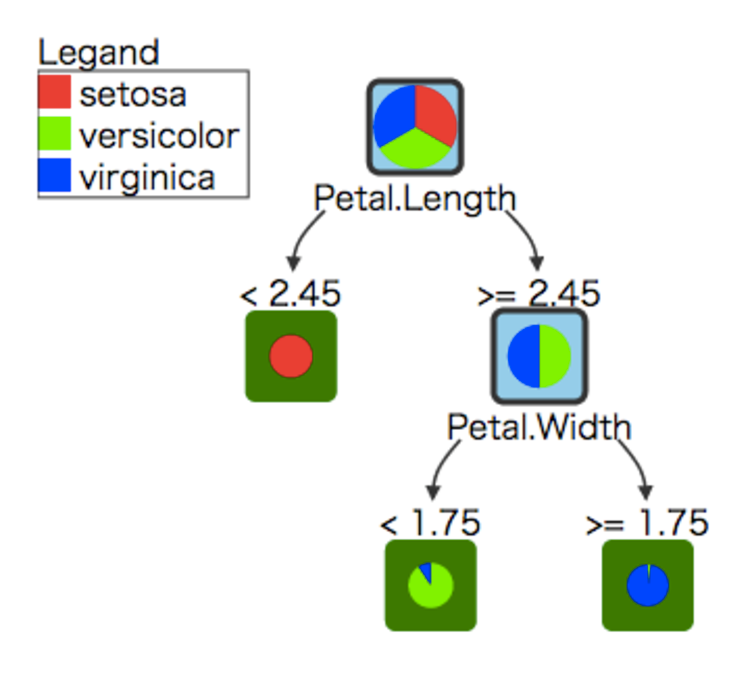
\includegraphics[scale=0.5]{figure/tree_3.eps}
\caption{アヤメデータセットの決定木\label{fig:mdtree_tree_3}}
\end{center}
\end{minipage}

\end{tabular}
\end{center}
\end{figure}

\begin{figure}[htbp]
\begin{center}
\begin{tabular}{c}

\begin{minipage}{0.5\hsize}
\begin{center}
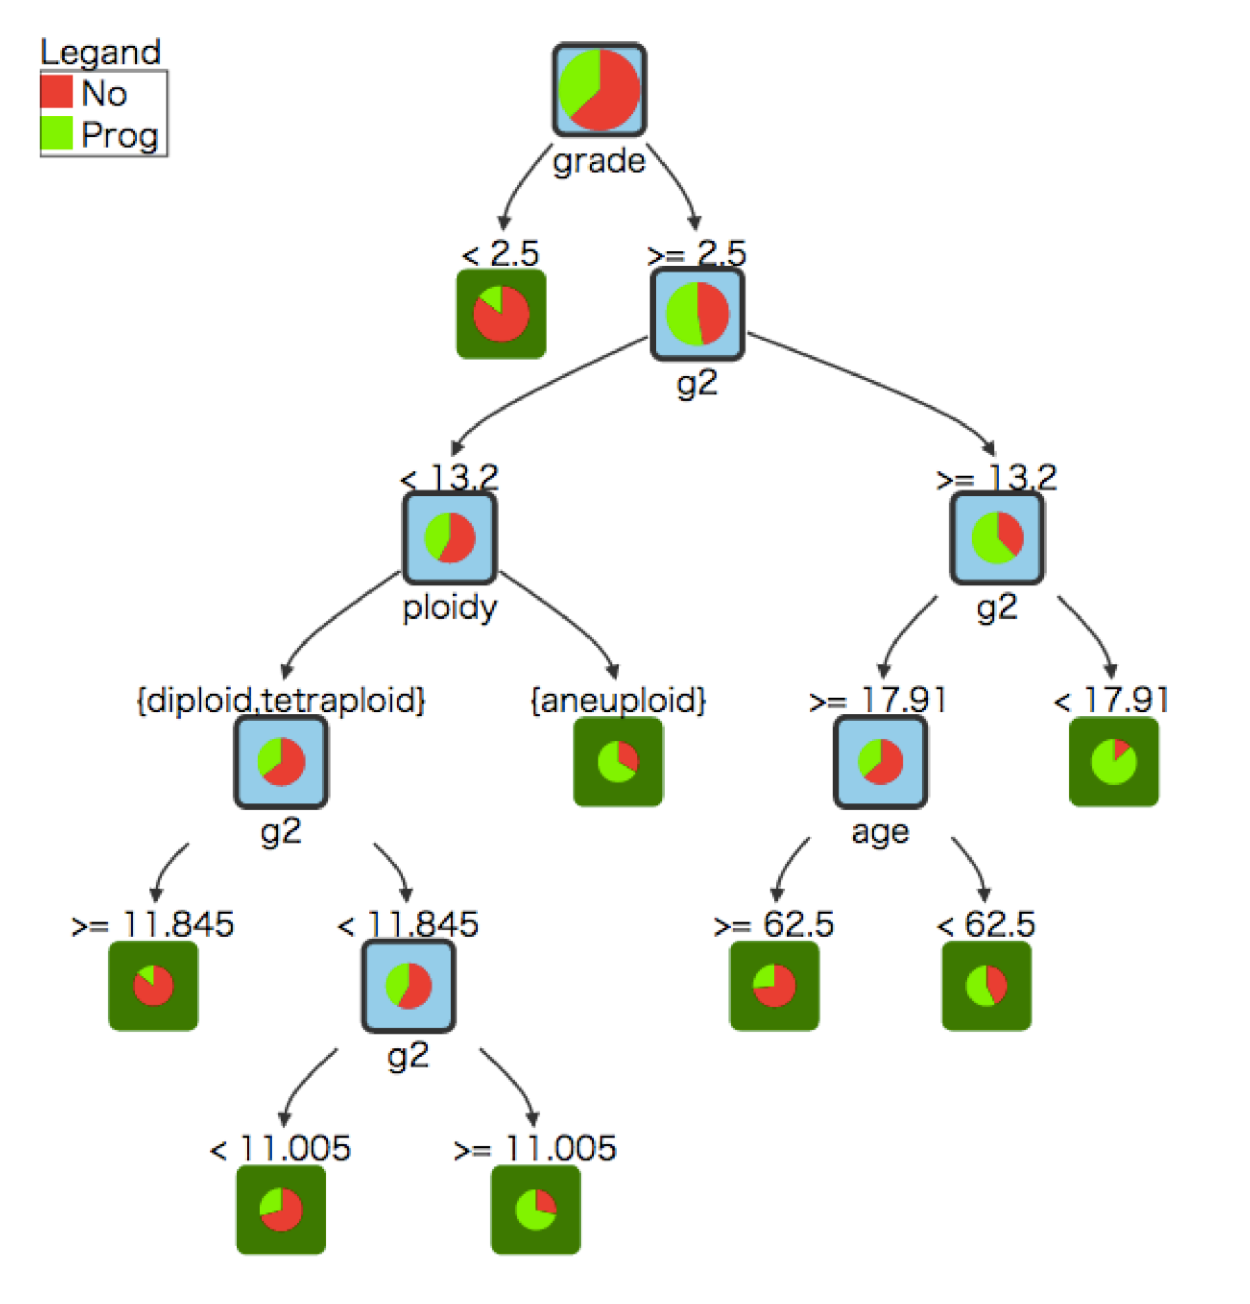
\includegraphics[scale=0.5]{figure/tree_4.eps}
\caption{前立腺がんの決定木\label{fig:mdtree_tree_4}}
\end{center}
\end{minipage}

\end{tabular}
\end{center}
\end{figure}



\subsection{書式}
\begin{verbatim}
mdtree.rb i= o= [alpha=] [--help]
\end{verbatim}

\begin{table}[htbp]
{\small
\begin{tabular}{ll}
\verb|i=| & : 決定木モデルのPMMLファイル \\
\verb|o=| & : 出力ファイル(HTMLファイル) \\
\verb|alpha=| & : 枝刈り度を指定する(0以上の実数で、大きくすると枝が多く刈られる)。 \\
              & : 指定しなかった場合、\verb|mbonsai|で交差検証を指定しなければ、\\
              & : 0.01が指定されたことになり、交差検証を指定していれば、誤分類率最小のモデルが描画される。\\
              & : このパラメータは\verb|mbonsai|で構築した決定木のみ有効。\\
\verb|--help| & : ヘルプの表示 \\
\end{tabular} 
}
\end{table} 

\subsection{利用例}
\subsubsection*{例1: Basic Example}

Example from the above section.


\begin{Verbatim}[baselinestretch=0.7,frame=single]
$ cat dat1.csv
gender,visitgap,purchasepattern,hospitalized
Male,1.2,ABCAAA,Yes
Male,10.5,BCDADD,Yes
Male,0.5,AAAA,No
Male,2.0,BBCC,No
Male,3.1,DEDDA,Yes
Female,0.7,CCCAA,No
Female,1.5,DDDEEE,Yes
Female,2.6,BACD,Yes
Female,3.5,ABBB,Yes
Female,4.0,DDDD,Yes
Female,2.1,DEDE,No
Male,1.2,ABCAAA,Yes
Male,10.5,BCDADD,Yes
Male,0.5,AAAA,No
Male,2.0,BBCC,No
Male,3.1,DEDDA,Yes
Male,0.7,CCCAA,No
Male,1.5,DDDEEE,No
Male,2.6,BACD,Yes
Male,3.5,ABBB,Yes
Male,4.0,DDDD,Yes
Male,2.1,DEDE,No
Male,1.2,ABCAAA,Yes
Male,10.5,BCDADDA,Yes
Male,0.5,AAAAA,No
Male,2.0,BBCCA,No
Male,3.1,DEDDA,Yes
Male,0.7,CCCAA,No
Male,1.5,ADDDEEE,Yes
Male,2.6,BACD,Yes
Male,3.5,ABBB,Yes
Male,4.0,DDDD,Yes
Female,2.1,DEDE,No
Female,1.2,ABCAAA,Yes
Female,10.5,BCDADD,Yes
Female,0.5,AAAA,No
Female,2.0,BBCC,No
Female,3.1,DEDDA,Yes
Female,0.7,CCCAA,No
Female,1.5,DDDEEE,Yes
Female,2.6,BACD,Yes
Female,3.5,ABBB,Yes
Female,4.0,DDDD,Yes
Female,2.1,DEDE,No
Female,1.2,ABCAAA,Yes
Female,10.5,BCDADD,Yes
Female,0.5,AAAA,No
Female,2.0,BBCC,No
Female,3.1,DEDDA,Yes
Female,0.7,CCCAA,No
Female,1.5,DDDEEE,Yes
Female,2.6,BACD,Yes
Female,3.5,ABBB,Yes
Female,1.0,DDDD,Yes
Female,2.5,DEDE,No
Female,2.5,ABBB,Yes
Female,1.0,DDDD,Yes
Female,1.1,DEDE,No
Female,2.2,ABCAAA,Yes
Female,10.5,BCDADD,Yes
Female,1.5,AAAA,No
Female,2.6,BBCC,No
Female,3.3,DEDDA,Yes
Female,1.7,CCCAA,No
Female,1.5,DDDEEE,Yes
Female,2.6,BACD,Yes
Female,3.9,ABBB,Yes
Female,4.5,DDDD,Yes
Female,2.1,DEDE,No
Female,3.9,BABB,Yes
Male,4.5,BAA,No
Female,2.1,DEDE,No
Male,3.9,BABB,Yes
Female,3.9,BABB,Yes
Male,4.5,BAA,No
Female,2.1,DEDE,No
Male,3.9,BABB,Yes
Female,3.9,BABB,Yes
Male,4.5,BAA,No
Female,2.1,DEDE,No
Male,3.9,BABB,Yes
$ mbonsai c=hospitalized n=visitgap p=purchasepattern d=gender i=dat1.csv O=outdat
ABCDE = 12345  *improved(errev:0.037037 *improved(errMin:0,leaf:1)
#END# kgbonsai O=outdat c=hospitalized d=gender i=dat1.csv n=visitgap p=purchasepattern
N=81
$ mdtree.rb i=outdat/model.pmml o=model1.html
#END# /usr/bin/mdtree.rb i=outdat/model.pmml o=model1.html
$ mdtree.rb alpha=0.1 i=outdat/model.pmml o=model2.html
#END# /usr/bin/mdtree.rb alpha=0.1 i=outdat/model.pmml o=model2.html
$ head model1.html
<html lang="ja">
<head>
  <meta charset="utf-8">
	<meta name="viewport" content="width=device-width, initial-scale=1.0">
  <style type="text/css">
	  p.title { border-bottom: 1px solid gray
		g > .type-node > rect { stroke-dasharray: 10,5
hite
		g > .type-leaf > rect { stroke-width: 3px
		.edge path {  fill: none
		svg >.legend > rect { stroke-width: 1px
$ head model2.html
<html lang="ja">
<head>
  <meta charset="utf-8">
	<meta name="viewport" content="width=device-width, initial-scale=1.0">
  <style type="text/css">
	  p.title { border-bottom: 1px solid gray
		g > .type-node > rect { stroke-dasharray: 10,5
hite
		g > .type-leaf > rect { stroke-width: 3px
		.edge path {  fill: none
		svg >.legend > rect { stroke-width: 1px
\end{Verbatim}


%\end{document}

